\documentclass{scrartcl}
\usepackage[utf8]{inputenc}

\usepackage{caption}
\usepackage{textcomp}
\usepackage{subcaption}
\usepackage{graphicx}

\title{Don't Panic: AV Edition}
\subtitle{NCPTW 2016}
\author{Matthew Moreno}

\begin{document}
\maketitle

\section{General Directives}
\begin{itemize}
  \item \textit{Stay calm!} Ninety-nine percent of the time, a simple solution will work every time.
  \item \textit{Use your millennial powers!} If you think you might know the solution to a problem, it will probably work. Try it. If you don't know the solution to a problem, Google it.
  \item \textit{Ask for Help!} Don't hesitate to contact the main desk to call in reinforcements.
  \item \textit{Don't Stress Out!} If something goes wrong, it's not your fault. You are doing your best to solve the problem. What you can do, you will and what you can't... you won't.
  \item \textit{Be Empathetic, But Firm} Presenters were warned that they should have planned to do their presentations on the conference laptops. Although we will try, the conference is not obligated to support presentations run on their personal computers.
\end{itemize}

\section{Cables}
Presenters should be using the conference-provided laptops to run their presentations (they have been warned about this!). These machines use VGA cables (Figure \ref{subfig:vga}) to connect to the projectors. If presenters wish to use their own computers to run their presentations, you may try to assist them. If their presentation is on a tablet, we may be able to accommodate them; there is a possibility that we will have iPad compatible-adapters on hand at the main desk. They will likely desire a HDMI connection (Figure \ref{subfig:hdmi}). Unfortunately, we do not have these cables. They might have a Mini Display port (especially if they are using an older-style Macintosh). The Mini Display cable is shown in Figure \ref{subfig:minidisplay}. We have a Mini Display to VGA adapter, which might be available at the main desk. Without an adapter, it is necessary to connect to our projectors using a VGA cable. Unfortunately, unless they brought their Clunktron 5000 Windows ME Edition, most folks are unlikely to have a VGA port on their computer. If they don't have a compatible port, they will need to transfer the presentation to a conference computer. This is covered in Section \ref{sec:transferring}. If they are able to connect their own machine, you will need to get their machine configured with the projector (Section \ref{sec:computer}).

\begin{figure}[h]
    \centering
    \begin{subfigure}[t]{0.25\textwidth}
        \centering
        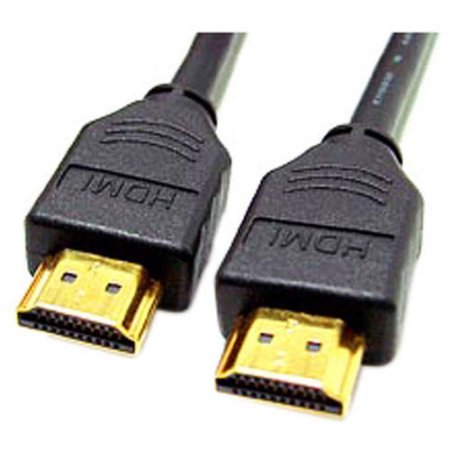
\includegraphics[width=\textwidth]{img/hdmi}
        \subcaption{HDMI}
        \label{subfig:hdmi}
    \end{subfigure}%
    \hfill 
    \begin{subfigure}[t]{0.25\textwidth}
        \centering
        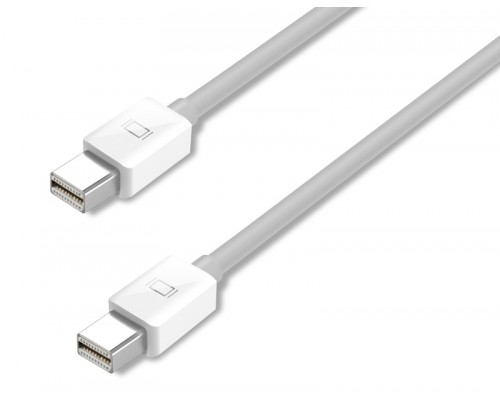
\includegraphics[width=\textwidth]{img/minidisplay}
        \subcaption{Mini DisplayPort}
        \label{subfig:minidisplay}
    \end{subfigure}%
    \hfill
    \begin{subfigure}[t]{0.25\textwidth}
        \centering
        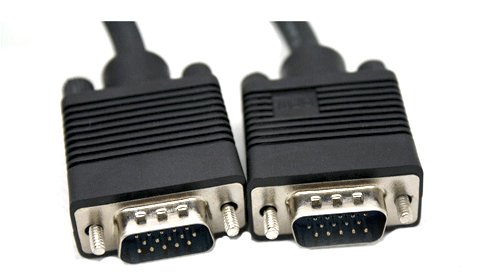
\includegraphics[width=\textwidth]{img/vga}
        \subcaption{VGA}
        \label{subfig:vga}
    \end{subfigure}%
    \hfill
    \begin{subfigure}[t]{0.25\textwidth}
        \centering
        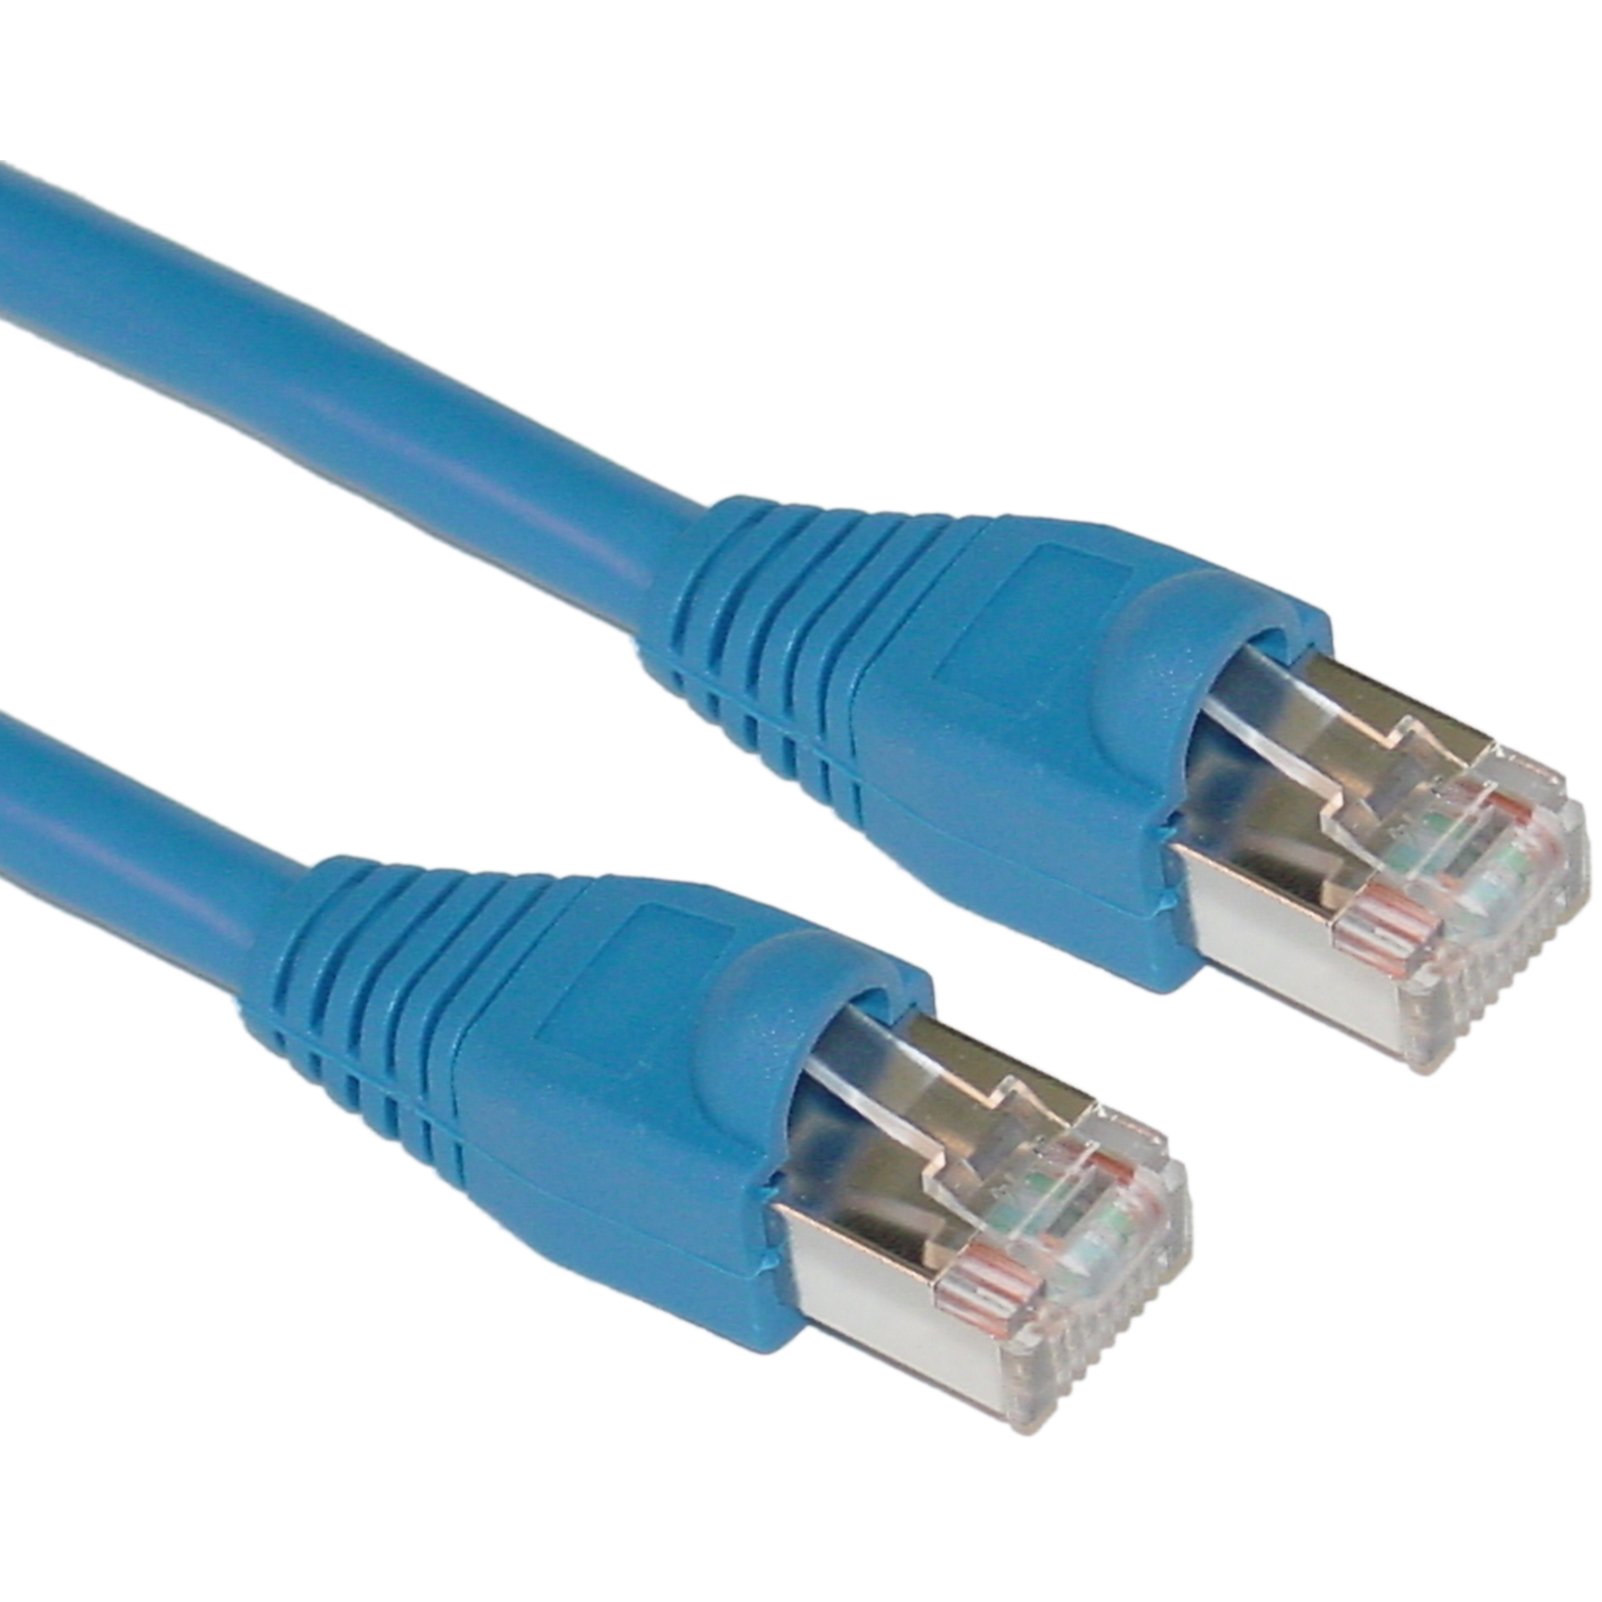
\includegraphics[width=\textwidth]{img/ethernet}
        \subcaption{Ethernet}
        \label{subfig:ethernet}
    \end{subfigure}%
    \caption{Three varieties of cabling you might encounter in the wild.}
    \label{fig:cables}
\end{figure}

\section{Configuring a Computer} \label{sec:computer}
Projectors often have multiple input sources. If the projector does not seem to recognize the computer you have plugged in, you should start out by checking to make sure that the proper input source is selected on the projector. Cycle through all the projector input sources, stopping at each for a few seconds. If no image shows up on the projection, try unplugging the cables, maybe blowing on them, and then reconnecting them. Cycle through the input sources again. If that still doesn't work, try it again. Cycle through the input sources once more. Then, try using different cables if there are any on hand. Cycle through the input source again. Double check to make sure that both the projector and the computer are powered on. Finally, check the computer display settings to make sure that the computer is sending output to the projector (see Listing \ref{fig:display_settings} for details).  If none of that works, contact the main desk for help. 

If the presenter would like to use present with notes in Powerpoint -- or expresses any other desire for content on the laptop screen to differ from content shown on the projected image -- you will need to configure the display settings to ``extend'' rather than ``mirror.'' Please refer to Listing \ref{fig:display_settings}. 

Finally, be sure to check that the computer being used to conduct the presentation is not set to auto sleep! See Listing \ref{fig:auto_sleep} for specific instructions on this topic.

\section{Configuring the Projector} \label{sec:projector}
The object of configuring the projector is to get the image to show up 
\begin{enumerate}
  \item at the right size, \label{item:size}
  \item in the right place, \label{item:place}
  \item not distorted, and \label{item:distorted}
  \item in focus. \label{item:focus}
\end{enumerate}

To accomplish Objective \ref{item:size}, use the scale control of the projector or position the projector closer to or further from the screen. To accomplish Objective \ref{item:place}, make sure that the projector is pointing at the screen; there are little feet on the bottom of the projector you can screw in or out to adjust the height of the projected image. To accomplish Objective \ref{item:distorted}, use the keystone control to adjust the ratio between the top of the image and the bottom (to make it more or less trapezoidal) and make sure that the projector is aiming head-on towards the screen. Finally, to accomplish Objective \ref{item:focus}, bring up some text on the display and fiddle with the focus control on the projector until the projected text appears sharp. This should be the last projector configuration step you take!

\section{Audio}
If the presenter would like to use audio during her talk, there are two sets of speakers available at the main desk. These speakers are USB-powered; you will need to plug them into a USB port in addition to the audio jack. Test the volume setting before the presentation to make sure that it is appropriate!

\section{Transferring A Presentation} \label{sec:transferring}
You should have a USB stick on hand. If not, several will be available at the main desk. The conference laptops run Microsoft Powerpoint. If the presenter's slides were created using different software (or even using Powerpoint on Mac), encourage the presenter to page through their presentation to make sure that it is rendered as they expected. If it doesn't render properly, see if the The conference laptops should also be able to handle PDF presentations. See Listing \ref{fig:pdf_presentation} for details on this topic.

Presenters may be using a web service such as Prezi or Google Slides. In this case, they will need internet access! Hopefully, Hotel Murano will provide adequate wireless internet access (wifi). If not, you will need to connect to via ethernet. If ethernet is available, jacks are likely to be located in the same kinds of places you would find power outlets -- look there for ethernet jacks. You will need an ethernet cable (Figure \ref{subfig:ethernet}). If one is not on hand, there should be one at the main desk. If both wifi and ethernet are unavailable, see if the presenter can download an offline version of their presentation (perhaps as a PDF? See Listing \ref{fig:pdf_presentation}).

\newpage
\section{Appendix}

\setcounter{figure}{0}    

\renewcommand{\figurename}{Listing}

\begin{figure}[h]
\caption{Configuring A Computer to Avoid Autosleep}
\begin{subfigure}[t]{0.5\textwidth}
\subcaption{Macintosh}
\begin{itemize}
\item \texttt{Apple} (upper left of menu bar)
\item \texttt{System Preferences...}
\item \texttt{Energy Saver}
\item Move the \texttt{Computer sleep} slider to \texttt{never}
\item save your changes
\end{itemize}
\end{subfigure}%
\hfill
\begin{subfigure}[t]{0.5\textwidth}
\subcaption{Windows}
\begin{itemize}
\item \texttt{Start}
\item \texttt{Control Panel}
\item \texttt{System and Security} or 
\item \texttt{System and Maintenance}
\item \texttt{Power Options}
\item \texttt{Change plan settings}
\item \texttt{Change advanced power settings}
\item \texttt{+} in front of \texttt{Sleep}
\item \texttt{+} in front of \texttt{Sleep after}
\item \texttt{Never} (for both \texttt{On Battery} and \texttt{Plugged In}
\item \texttt{+} in front of \texttt{Hibernate after}
\item \texttt{Never} (for both \texttt{On Battery} and \texttt{Plugged In}
\item save your changes
\end{itemize}
\end{subfigure}
\label{fig:auto_sleep}
\addtocounter{figure}{-1} 
\end{figure}

\begin{figure}[h] 
\caption{Working with Computer Display Settings}
\begin{subfigure}[t]{0.5\textwidth}
\subcaption{Macintosh}
\begin{itemize}
\item \texttt{Apple} (upper left of menu bar)
\item \texttt{System Preferences...}
\item \texttt{Displays}
\item \texttt{Arrangement}
\item select desired setting
\end{itemize}
\end{subfigure}%
\hfill
\begin{subfigure}[t]{0.5\textwidth}
\subcaption{Windows}
\begin{itemize}
\item Press \texttt{windows}-\texttt{p}
\item select desired setting
\end{itemize}
\end{subfigure}
\label{fig:display_settings}
\addtocounter{figure}{-1} 
\end{figure}

\begin{figure}[h] 
\caption{Running a PDF Presentation on a Conference Laptop}
\begin{itemize}
\item \texttt{open} their presentation using Adobe Acrobat Reader DC
\item \texttt{ctrl-l} to enter presentation mode
\item during the presentation...
\begin{itemize}
	\item next page: \texttt{click} anywhere or \texttt{\textrightarrow}
	\item previous page: \texttt{shift}-\texttt{click} anywhere or \texttt{\textleftarrow}
	\item beginning of the document: \texttt{Home}
	\item end of the document: \texttt{End}
\end{itemize}
\item exit presentation mode: \texttt{Esc}
\end{itemize}
\label{fig:pdf_presentation}
\end{figure}
\end{document}
